% \documentclass[sigconf,anonymous,review]{acmart}
\documentclass[sigconf]{acmart}

%% Rights management information.  This information is sent to you
%% when you complete the rights form.  These commands have SAMPLE
%% values in them; it is your responsibility as an author to replace
%% the commands and values with those provided to you when you
%% complete the rights form.
\setcopyright{acmcopyright}
\copyrightyear{2023}
\acmYear{2023}
\acmDOI{XXXXXXX.XXXXXXX}

%% These commands are for a PROCEEDINGS abstract or paper.
\acmConference[Conference acronym 'XX]{Conference title}{January 01--02,
  1900}{Someplace, NY}
\acmPrice{15.00}
\acmISBN{978-1-4503-XXXX-X/18/06}

%%
%% Submission ID.
%% Use this when submitting an article to a sponsored event. You'll
%% receive a unique submission ID from the organizers
%% of the event, and this ID should be used as the parameter to this command.
\acmSubmissionID{123-A56-BU3}

%%
%% The majority of ACM publications use numbered citations and
%% references.  The command \citestyle{authoryear} switches to the
%% "author year" style.
%%
%% If you are preparing content for an event
%% sponsored by ACM SIGGRAPH, you must use the "author year" style of
%% citations and references.
%% Uncommenting
%% the next command will enable that style.
\citestyle{acmauthoryear}


\begin{document}

\title{Coevolution of Camouflage}

%% Authors
\author{Craig Reynolds}
\email{cwr@red3d.com}
\orcid{0000-0001-8203-712X}
\affiliation{%
  \institution{unaffiliated researcher}
  \country{USA}
}

\renewcommand{\shortauthors}{Craig Reynolds}

\begin{abstract}
  [... super preliminary ... an abstract model of the evolution of camouflage in nature through adversarial interaction between predator and prey ... model contains representation of populations of predator and prey ...]
  [... produces camouflage textures for given backgrounds (typically photos of the real world) based on mutual conflict between predators and prey]
\end{abstract}

%%
%% Generate your CCSCML using http://dl.acm.org/ccs.cfm.
%%
\begin{CCSXML}
<ccs2012>
   <concept>
       <concept_id>10010147.10010341.10010349.10011810</concept_id>
       <concept_desc>Computing methodologies~Artificial life</concept_desc>
       <concept_significance>500</concept_significance>
       </concept>
   <concept>
       <concept_id>10010147.10010371.10010382.10010384</concept_id>
       <concept_desc>Computing methodologies~Texturing</concept_desc>
       <concept_significance>500</concept_significance>
       </concept>
   <concept>
       <concept_id>10010147.10010178.10010224</concept_id>
       <concept_desc>Computing methodologies~Computer vision</concept_desc>
       <concept_significance>500</concept_significance>
       </concept>
    
    <concept>
        <concept_id>10010147.10010257.10010293.10011809.10011813</concept_id>
        <concept_desc>Computing methodologies~Genetic programming</concept_desc>
        <concept_significance>500</concept_significance>
    </concept>
 </ccs2012>
\end{CCSXML}

\ccsdesc[500]{Computing methodologies~Artificial life}
\ccsdesc[500]{Computing methodologies~Texturing}
\ccsdesc[500]{Computing methodologies~Computer vision}
\ccsdesc[500]{Computing methodologies~Genetic programming}

%% Keywords
\keywords{camouflage, coevolution, nature, biology, predator, prey, vision, texture synthesis}

%% Teaser figure that appears on the top of the article.
\begin{teaserfigure}
    %% TODO note that these are all the same image, and for this figure I probably
    %% want to use images without the “predator prediction crosshairs”.
    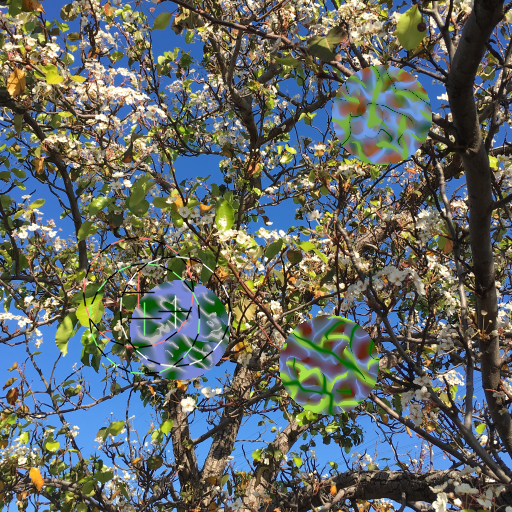
\includegraphics[scale=0.24]{images/20220926_step_6143.png}
    \hfill
    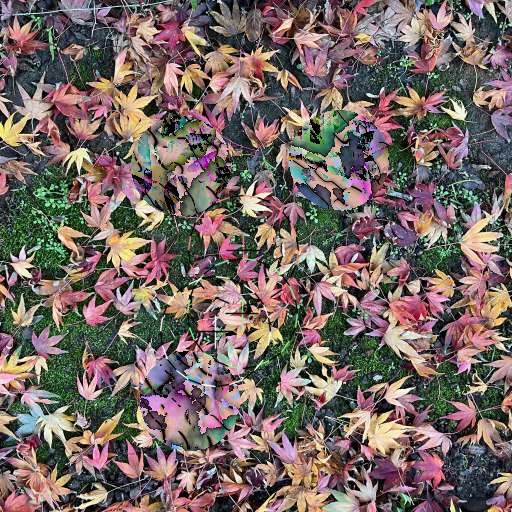
\includegraphics[scale=0.24]{images/20220918_step_7372.png}
    \hfill
    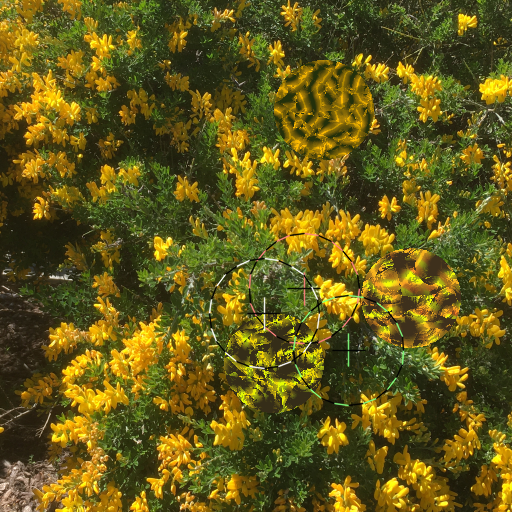
\includegraphics[scale=0.24]{images/20220930_step_6093.png}
    \hfill
    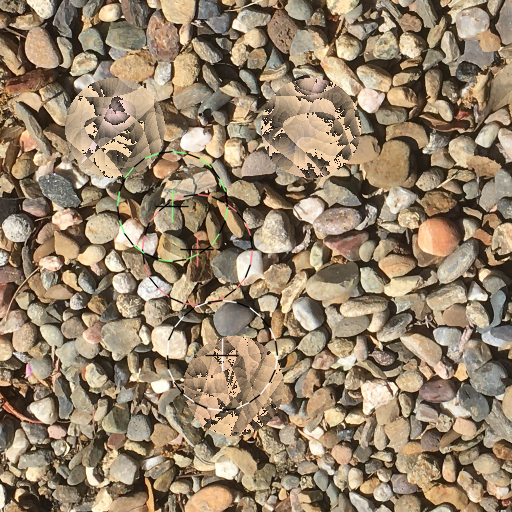
\includegraphics[scale=0.24]{images/20221003_step_3667.png}
    \caption{Circular \textit{prey} each with an evolved camouflage patterns, overlaid on photographs of real world textures. Each image contains three prey.}
    \Description{Examples of camouflage textures produced by the simulation.}
    \label{fig:teaser}
    \vspace{5mm} %5mm vertical space
\end{teaserfigure}

%% I guess this lays out the single column “top matter” defined above.
\maketitle

\section{Introduction}
This work aims to create a simplified and abstract 2d simulation model of the evolution of camouflage textures in nature. These camouflage patterns emerge in the interaction, the coevolution, of a population of \textit{prey} each with a candidate texture and a population of \textit{predators} each with a learned visual detector. The input to the simulation is a set of photos of a background environment. The prey evolve to be \textit{cryptic} — hard to see — against the background images. The predators evolve and learn to hunt the prey by locating their position within the environment.

Computational models of complex biological systems have several benefits. Constructing them, getting them to work as seen in nature, helps crystallize our thinking about natural phenomenon. Computational models also allow experimentation \textit{in silico} to help characterize this complex natural systems.

[... introduction ... following the approach of \citet{Reynolds2011} a population of prey, each with a synthetic camouflage texture, are evolved against negative selection by a predator which prefers the most conspicuous prey against a given background. ...]

\section{Related work}
[... xxx ...]

[... TexSyn is based on the “strongly typed” variant of Genetic Programming known as STGP \cite{montana_strongly_1995}, one of several grammar-based GP variants \cite{Mckay_2010}. ...]

%% Acknowledgements
\begin{acks}
[... Many thanks to all who helped me with this work: my supportive family, Andrew Glassner for teaching me everything I know about deep learning, Ken Perlin for, lots but especially [An Image Synthesizer?] Pat Hanrahan for helpful career advice (“just do the research”). ...]

[maybe just names: 
Ken Perlin
Pat Hanrahan
Karl Sims
Andrew Glassner
Richard Dawkins
Peter Angeline 
Jordan Pollack
]
\end{acks}

%% Bibliography.
\bibliographystyle{ACM-Reference-Format}
\bibliography{coc.bib}

%% Appendix
\appendix

\section{Additional Section}
Text

% Note (from https://s2022.siggraph.org/technical-papers-submissions-faq/): 
% The Conference Paper track encourages submissions for high-quality, 
% ground-breaking research that fits within a strict 7-page limit (plus 
% additional pages for references), and may be more appropriate for
% research that is less-polished but still potentially-impactful. Journal 
% papers do not have a page limit, and may include more thorough experiments
% and derivations within the main paper. 

\end{document}
